% =========================================================================
% Capítulo 1 - Tema 01: Cinemática en Coordenadas Cilíndricas
% =========================================================================

\section{Tema 01: Cinemática en Coordenadas Cilíndricas}

En este tema estudiamos el movimiento de puntos expresado en coordenadas cilíndricas.
Este sistema es natural para problemas con simetría axial o movimiento rotacional.

\subsection{Ejercicios}

\subsubsection{Hormiga velocista}
En la figura \ref{fig:Hormiga}, se encuentra una hormiga (Punto $B$), la cual camina de manera radial, hacia afuera del disco a una velocidad constante $v_0$ desde el centro. Si el disco rota desde su centro $O$ con una velocidad angular de magnitud $\Omega$ relativa al suelo, determine:
\begin{enumerate}
    \item La posición con respecto al tiempo.
    \item La velocidad con respecto al tiempo.
    \item La aceleración con respecto al tiempo.
\end{enumerate}

\begin{figure}[!ht]
    \centering
\begin{tikzpicture}[>=Latex, scale=1.5]

    % --- CONFIGURACIÓN DE DIMENSIONES ---
    \def\R{3}      % Radio mayor de la elipse (ancho)
    \def\r{0.8}    % Radio menor de la elipse (alto/perspectiva)
    \def\h{0.15}   % Grosor del disco
    \def\Hshaft{1.2} % Largo del eje

    % 1. EJE CENTRAL (PARTE INFERIOR)
    % Dibujamos el cilindro del eje debajo del disco
    \fill[gray!60] (-0.4, -\h) rectangle (0.4, -\Hshaft);
    \draw[thick] (-0.4, -\h) -- (-0.4, -\Hshaft);
    \draw[thick] (0.4, -\h) -- (0.4, -\Hshaft);
    \draw[thick, fill=gray!70] (0, -\Hshaft) ellipse (0.4 and 0.15);

    % 2. GROSOR DEL DISCO (BORDE LATERAL)
    % Se dibuja la mitad inferior de la elipse desplazada hacia abajo
    \fill[gray!50] (\R, 0) arc (0:-180:\R\space and \r) -- (-\R, -\h) arc (-180:0:\R\space and \r) -- cycle;
    \draw[thick] (\R, 0) arc (0:-180:\R\space and \r);
    \draw[thick] (\R, -\h) arc (0:-180:\R\space and \r);
    \draw[thick] (\R, 0) -- (\R, -\h);
    \draw[thick] (-\R, 0) -- (-\R, -\h);

    % 3. SUPERFICIE SUPERIOR DEL DISCO
    \draw[thick, fill=gray!20] (0,0) ellipse [x radius=\R, y radius=\r];

    % 4. PUNTOS Y VECTORES
    % Punto O (Centro)
    \coordinate (O) at (0,0);
    \filldraw (O) circle (1.5pt) node[left, xshift=-2pt] {$O$};

    % Punto B (Partícula) - Calculado para que parezca estar sobre la elipse
    % Usamos coordenadas polares modificadas por la proporción de la elipse
    \def\ang{20} % Ángulo de posición
    \def\dist{2.0} % Distancia radial r
    \coordinate (B) at ({\dist*cos(\ang)}, {\dist*sin(\ang)*(\r/\R)});

    % Dibujo del grupo de puntos B
    \filldraw (B) circle (1.5pt);

    \node[below right] at (B) {$B$};

    % Vector r (Posición)
    \draw[->, thick] (O) -- (B) node[midway, above] {$r$};

    % Vector v0 (Velocidad tangencial)
    % El ángulo de v0 debe seguir la inclinación de la elipse (tangente)
    \draw[->, very thick, blue] (B) -- ++({0.8*cos(\ang)}, {0.8*sin(\ang)*(\r/\R)}) node[below] {$v_0$};

    % 5. INDICADOR DE ROTACIÓN OMEGA
    \draw[->, thick] (-0.6, 0) arc (170:370:0.6 and 0.2);
    \node[left] at (-0.7, -0) {$\Omega$};

\end{tikzpicture}
    \caption{Hormiga Velocista}
    \label{fig:Hormiga}
\end{figure}
\subsubsection{Movimiento en coordenadas cilíndricas}

Se observa una partícula en movimiento con respecto a un sistema de referencia inercial. La trayectoria está dada por las siguientes funciones:
\[ r = Ae^{k\theta}, \quad z = hr \]
donde $r, \theta$ y $z$ son coordenadas cilíndricas, siendo $A, k$ y $h$ valores escalares constantes y mayores que cero, como se muestra en la Figura \ref{fig:c1_e01_p02_espiral_cilindricas}. Suponiendo que su rapidez es constante ($v_0$) y conocida:

\begin{enumerate}
    \item Calcule la velocidad $\vec{v}$ de la partícula en función de $\theta, A, k, h$ y $v_0$.
    \item Encuentre su aceleración $\vec{a}$ en función de los mismos parámetros.
    \item Pruebe que $\vec{a} \perp \vec{v}$.
    \item Encuentre una expresión para $\theta(t)$.
\end{enumerate}

% Figura principal
\begin{figure}[!ht]
    \centering
    \begin{tikzpicture}[>=Latex, scale=1.5]

        % --- CONFIGURACIÓN DE PARÁMETROS ---
        \def\A{0.15}      % Constante A de la espiral [u]
        \def\k{0.22}      % Constante k (crecimiento) [-]
        \def\thP{560}     % Ángulo del punto P [deg] (una vuelta y media)
        \def\thPmod{200}  % Azimut equivalente de P [deg]

        % --- SISTEMAS DE COORDENADAS ---
        \draw[->, thick, gris1] (-2.2,0) -- (2.4,0) node[below right] {$x$};
        \draw[->, thick, gris1] (0,-1.8) -- (0,2.2) node[left] {$y$};

        % --- GEOMETRÍA PRINCIPAL ---
        % Espiral logarítmica r = A e^{k theta} (vista superior)
        \draw[thick, gris1, domain=0:720, samples=300, smooth, variable=\t]
            plot ({\t}:{\A*exp(\k*\t/57.29578)});

        % --- PUNTOS Y COORDENADAS ---
        \pgfmathsetmacro{\rP}{\A*exp(\k*\thP/57.29578)}
        \coordinate (O) at (0,0);
        \coordinate (P) at (\thP:\rP);
        \draw[mydashed, gris1!60] (O) -- (P);

        % --- VECTORES Y FUERZAS ---
        % Vectores unitarios cilíndricos en P
        \draw[->, very thick, myred] (P) -- ++(\thP:0.55) node[above left] {$\hat{e}_r$};
        \draw[->, very thick, myred] (P) -- ++(\thP+90:0.55) node[below left] {$\hat{e}_\theta$};
        % Velocidad (tangente a la espiral, rapidez constante v0)
        \pgfmathsetmacro{\alphat}{atan(1/\k)}
        \draw[->, very thick, azul] (P) -- ++(\thP+\alphat:0.9) node[below] {$\vec{v}$};

        % --- ANOTACIONES Y ETIQUETAS ---
        \fill[gris1] (P) circle (1.2pt) node[above right, xshift=1pt] {$P$};
        \node[below left] at (O) {$O$};
        \draw[->] (0.35,0) arc (0:\thPmod:0.35);
        \node at ({\thPmod/2}:0.55) {$\theta$};
        \node[gris1] at (1.6,-1.4) {$r = Ae^{k\theta}$};

    \end{tikzpicture}
    \caption{Vista superior de la espiral $r=Ae^{k\theta}$; la altura crece como $z=hr$}
    \label{fig:c1_e01_p02_espiral_cilindricas}
\end{figure}


\subsubsection{Sistema de doble varilla}
Dos varillas rígidas de longitudes $l_1$ y $l_2$ están articuladas en serie como se muestra en la Figura \ref{fig:doble_varilla}. La varilla $OA$ está articulada en uno de sus extremos al punto fijo $O$, mientras que su otro extremo está articulado en el punto $A$, que es un extremo de la segunda varilla $AP$. El punto $P$ se encuentra en el extremo libre de la varilla $AP$. Sabiendo que $\theta$ es el ángulo entre la varilla $OA$ y la horizontal y que $\phi$ es el ángulo entre la varilla $AP$ y la prolongación de la varilla $OA$, determine:

\begin{enumerate}
    \item La velocidad y aceleración del punto $P$ vistas por un observador fijo a la varilla $OA$.
    \item La velocidad y aceleración del punto $P$ vistas por un observador fijo al suelo.
\end{enumerate}

\begin{figure}[htbp]
    \centering
    \begin{tikzpicture}[>=Latex, scale=1.5]
        % --- Parámetros Geométricos ---
        \def\Lone{2.8}     % Longitud l1
        \def\Ltwo{2.0}     % Longitud l2
        \def\ThetaAng{25}  % Ángulo theta
        \def\PhiAng{35}    % Ángulo phi relativo a OA

        % --- 1. Soporte y Suelo en O ---
        \coordinate (O) at (0,0);
        \draw[thick] (-0.4,-0.4) -- (0.4,-0.4);
        \fill[pattern=north east lines] (-0.4,-0.5) rectangle (0.4,-0.4);
        \draw (O) -- (-0.2,-0.4);
        \draw (O) -- (0.2,-0.4);
        \filldraw[fill=white] (O) circle (2.5pt) node[left, xshift=-2pt] {$O$};

        % --- 2. Varilla OA ---
        \coordinate (A) at ({\ThetaAng}:\Lone);
        % Dibujo de la varilla con estilo 2D
        \draw[line width=5pt, color=gray!20, line cap=round] (O) -- (A);
        \draw[thick] (O) -- (A);
        \filldraw[fill=white] (A) circle (2pt) node[below right] {$A$};
        \node[above left] at ($(O)!0.5!(A)$) {$l_1$};

        % --- 3. Varilla AP ---
        % El ángulo absoluto de AP es (Theta + Phi)
        \coordinate (P) at ($(A) + ({\ThetaAng + \PhiAng}:\Ltwo)$);
        \draw[line width=5pt, color=gray!20, line cap=round] (A) -- (P);
        \draw[thick] (A) -- (P);
        \filldraw (P) circle (1.5pt) node[above right] {$P$};
        \node[above left] at ($(A)!0.5!(P)$) {$l_2$};

        % --- 4. Ángulos y Referencias ---
        % Ángulo theta
        \draw[dashed] (O) -- (1.5,0);
        \draw[->] (0.8,0) arc (0:\ThetaAng:0.8);
        \node at (1.0, 0.2) {$\theta$};

        % Ángulo phi (respecto a la prolongación de OA)
        \coordinate (Prolong) at ($(A) + ({\ThetaAng}:1.2)$);
        \draw[dashed] (A) -- (Prolong);
        \draw[->] ($(A) + ({\ThetaAng}:0.7)$) arc (\ThetaAng:{\ThetaAng+\PhiAng}:0.7);
        \node at ($(A) + ({\ThetaAng + 0.5*\PhiAng}:0.95)$) {$\phi$};

    \end{tikzpicture}
    \caption{Sistema de doble varilla articulada con longitudes $l_1$ y $l_2$, donde se definen los ángulos $\theta$ y $\phi$ para el análisis cinemático.}
    \label{fig:doble_varilla}
\end{figure}
\subsubsection{Collarín en brazo rotatorio}
Un collarín se desliza libremente a lo largo de un brazo rígido, como se muestra en la Figura \ref{fig:collarin_brazo}. El brazo está articulado en uno de sus extremos a un punto $O$, el cual está fijo al suelo, y rota alrededor de una dirección que es ortogonal al plano de movimiento.

Sabiendo que la posición del collarín está descrita por las variables $r$ y $\theta$, donde $r$ es el desplazamiento del collarín relativo al punto $O$ y $\theta$ es el ángulo de la barra medido con respecto a una dirección fija al suelo, determine lo siguiente para un observador fijo al suelo:

\begin{enumerate}
    \item El vector velocidad del collarín.
    \item El vector aceleración del collarín.
    \item La aceleración angular del collarín.
\end{enumerate}

\begin{figure}[!ht]
    \centering
    \begin{tikzpicture}[>=Latex, scale=1.5]
        \def\ang{35} \def\rPos{3.0}
        \coordinate (O) at (0,0);
        \fill[pattern=north east lines] (-0.5,-0.5) rectangle (0.5,-0.4);
        \draw[thick] (-0.5,-0.4) -- (0.5,-0.4);
        \draw (O) -- (-0.25,-0.4);
        \draw (O) -- (0.25,-0.4);
        \filldraw[fill=white] (O) circle (3pt) node[above left] {$O$};
        \coordinate (End) at (\ang:4.5);
        \draw[line width=7pt, color=black,cap=round] (O) -- (End);
        \draw[line width=6pt, color=gray!20,cap=round] (O) -- (End);
        \draw[thick] (O) -- (End);
        
        % COLLARÍN CON DEGRADADO CORREGIDO
        \coordinate (P) at (\ang:\rPos);
        \node[
            top color=gray!5, 
            bottom color=gray!60, 
            draw=black, 
            thick, 
            shape=rounded rectangle, 
            minimum width=0.6cm, 
            minimum height=0.35cm, 
            rotate=\ang+90, 
            inner sep=0pt
        ] at (P) {};
        \filldraw (P) circle (1.2pt) node[above, yshift=6pt] {$P$};

        \draw[dashed] (O) -- (2,0);
        \draw[->] (1,0) arc (0:\ang:1) node[midway, right, xshift=2pt] {$\theta$};
        \draw[|->] ($(O)+(90+\ang:0.4)$) -- ($(P)+(90+\ang:0.4)$) node[midway, above left] {$r$};
        \filldraw[fill=black] (O) circle (1pt);
    \end{tikzpicture}
    \caption{Collarín deslizando sobre un brazo rotatorio.}
    \label{fig:collarin_brazo}
\end{figure}
\ifmostrarSolucion
\begin{tcolorbox}[title= SOlucion Collarian brazo rotatorio, breakable]
\noindent\textbf{Primero, definimos los marcos de referencia y sistemas de coordenadas:}

\vspace{0.3cm}

\noindent $\mathcal{F}$: Suelo (Inercial) \quad $\{\vec{E}_x, \vec{E}_y, \vec{E}_z\}$ \\
\noindent $\mathcal{A}$: Fijo en el brazo \quad $\{\vec{e}_r, \vec{e}_\theta, \vec{e}_z\}$

\vspace{0.5cm}

% --- DIAGRAMA TIKZ Y RELACIONES DE TRANSFORMACIÓN ---
\noindent
\begin{minipage}{0.55\textwidth}
\centering
\begin{tikzpicture}[scale=1.2, >=stealth]
   \def\ang{35} \def\rPos{3.0}
        \coordinate (O) at (0,0);
        \fill[pattern=north east lines] (-0.5,-0.5) rectangle (0.5,-0.4);
        \draw[thick] (-0.5,-0.4) -- (0.5,-0.4);
        \draw (O) -- (-0.25,-0.4);
        \draw (O) -- (0.25,-0.4);
        \filldraw[fill=white] (O) circle (3pt) node[above left] {$O$};
        \coordinate (End) at (\ang:4.5);
        \draw[line width=7pt, color=black,cap=round] (O) -- (End);
        \draw[line width=6pt, color=gray!20,cap=round] (O) -- (End);
        \draw[thick] (O) -- (End);
        
        % COLLARÍN CON DEGRADADO CORREGIDO
        \coordinate (P) at (\ang:\rPos);
        \node[
            top color=gray!5, 
            bottom color=gray!60, 
            draw=black, 
            thick, 
            shape=rounded rectangle, 
            minimum width=0.6cm, 
            minimum height=0.35cm, 
            rotate=\ang+90, 
            inner sep=0pt
        ] at (P) {};
        \filldraw (P) circle (1.2pt) node[above, yshift=6pt] {$P$};

        \draw[dashed] (O) -- (2,0);
        \draw[->] (1,0) arc (0:\ang:1) node[midway, right, xshift=2pt] {$\theta$};
        \draw[|->] ($(O)+(90+\ang:0.4)$) -- ($(P)+(90+\ang:0.4)$) node[midway, above left] {$r$};
        \filldraw[fill=black] (O) circle (1pt);

  % Marco Inercial F (Morado)
  \draw[->, line width=1.2pt, violet] (0,0) -- (2.5,0) node[right] {$\vec{E}_x$};
  \draw[->, line width=1.2pt, violet] (0,0) -- (0,2.5) node[above] {$\vec{E}_y$};
  \node[violet] at (-0.25,0.15) {$\vec{E}_z$};

  % Vector unitario e_theta (Verde)
  \draw[->, line width=1.2pt, green!60!black] (0,0) -- ({2.0*cos(\ang)},{2.0*sin(\ang)}) node[above left] {$\vec{e}_r$};
  \draw[->, line width=1.2pt, green!60!black] (0,0) -- ({2.0*cos(\ang+90)},{2.0*sin(\ang+90)}) node[above left] {$\vec{e}_\theta$};
  \node[green!60!black] at (-0.35,-0.1) {$\vec{e}_z$};
\end{tikzpicture}
\end{minipage}
\begin{minipage}{0.42\textwidth}
\[
\begin{aligned}
\vec{e}_r &= \cos\theta \vec{E}_x + \sin\theta \vec{E}_y \\
\vec{e}_\theta &= -\sin\theta \vec{E}_x + \cos\theta \vec{E}_y \\
\vec{e}_z &= \vec{E}_z
\end{aligned}
\]
\end{minipage}

\vspace{0.8cm}

% --- PARTE A ---
\noindent\textbf{A) Definamos:} 
\[
\vec{r} = r\vec{e}_r, \qquad {}^{\mathcal{F}}\vec{\omega}^{\mathcal{A}} = \dot{\theta}\vec{e}_z
\]

\[
\Rightarrow {}^{\mathcal{F}}\vec{v} = \frac{{}^{\mathcal{F}}d}{dt}\vec{r} = \frac{{}^{\mathcal{A}}d}{dt}\vec{r} + {}^{\mathcal{F}}\vec{\omega}^{\mathcal{A}} \times \vec{r} \quad \text{(Teorema de Transporte)}
\]

\begin{itemize}
    \item $\frac{{}^{\mathcal{A}}d}{dt}\vec{r} = \dot{r}\vec{e}_r$
    \item ${}^{\mathcal{F}}\vec{\omega}^{\mathcal{A}} \times \vec{r} = \dot{\theta}\vec{e}_z \times r\vec{e}_r = r\dot{\theta}\vec{e}_\theta$
\end{itemize}

\[
\Rightarrow \boxed{{}^{\mathcal{F}}\vec{v} = \dot{r}\vec{e}_r + r\dot{\theta}\vec{e}_\theta}
\]

\[
\Rightarrow {}^{\mathcal{F}}\vec{a} = \frac{{}^{\mathcal{F}}d}{dt}({}^{\mathcal{F}}\vec{v}) = \frac{{}^{\mathcal{A}}d}{dt}({}^{\mathcal{F}}\vec{v}) + {}^{\mathcal{F}}\vec{\omega}^{\mathcal{A}} \times {}^{\mathcal{F}}\vec{v}
\]

\[
\left.
\begin{aligned}
\cdot \; \frac{{}^{\mathcal{A}}d}{dt}({}^{\mathcal{F}}\vec{v}) &= \ddot{r}\vec{e}_r + (\dot{r}\dot{\theta} + r\ddot{\theta})\vec{e}_\theta \\[4pt]
\cdot \; {}^{\mathcal{F}}\vec{\omega}^{\mathcal{A}} \times {}^{\mathcal{F}}\vec{v} &= \dot{\theta}\vec{e}_z \times (\dot{r}\vec{e}_r + r\dot{\theta}\vec{e}_\theta) \\
&= \dot{r}\dot{\theta}\vec{e}_\theta - r\dot{\theta}^2\vec{e}_r
\end{aligned}
\right\} 
\Rightarrow \boxed{{}^{\mathcal{F}}\vec{a} = (\ddot{r} - r\dot{\theta}^2)\vec{e}_r + (2\dot{r}\dot{\theta} + r\ddot{\theta})\vec{e}_\theta}
\]

\vspace{0.8cm}

% --- PARTE B ---
\noindent\textbf{B) Definamos:}

\[
\frac{{}^{\mathcal{F}}d}{dt}(\vec{e}_r) = -\dot{\theta}\sin\theta \vec{E}_x + \dot{\theta}\cos\theta \vec{E}_y = \dot{\theta}\vec{e}_\theta
\]
\[
\frac{{}^{\mathcal{F}}d}{dt}(\vec{e}_\theta) = -\dot{\theta}\cos\theta \vec{E}_x - \dot{\theta}\sin\theta \vec{E}_y = -\dot{\theta}\vec{e}_r
\]

\begin{itemize}
    \item $\vec{r} = r\vec{e}_r$
    \item ${}^{\mathcal{F}}\vec{v} = \frac{{}^{\mathcal{F}}d}{dt}(\vec{r}) = \dot{r}\vec{e}_r + r\dot{\theta}\vec{e}_\theta$
    \item ${}^{\mathcal{F}}\vec{a} = \frac{{}^{\mathcal{F}}d}{dt}({}^{\mathcal{F}}\vec{v}) = \ddot{r}\vec{e}_r + \dot{r}\dot{\theta}\vec{e}_\theta + \dot{r}\dot{\theta}\vec{e}_\theta + r\left[\ddot{\theta}\vec{e}_\theta - \dot{\theta}^2\vec{e}_r\right]$
    \[
    = \ddot{r}\vec{e}_r + \dot{r}\dot{\theta}\vec{e}_\theta + \dot{r}\dot{\theta}\vec{e}_\theta + r\ddot{\theta}\vec{e}_\theta - r\dot{\theta}^2\vec{e}_r
    \]
    \[
    = (\ddot{r} - r\dot{\theta}^2)\vec{e}_r + (2\dot{r}\dot{\theta} + r\ddot{\theta})\vec{e}_\theta
    \]
\end{itemize}

    
\end{tcolorbox}
\fi

\subsubsection{Barra articulada a argolla circular}

Una barra (con espesor mayor que cero) de longitud $\ell$ está articulada en uno de sus extremos a una argolla, como se muestra en la Figura \ref{fig:barra_anillo}. La argolla se desliza a lo largo de una pista fija en forma de anillo circular de radio $R$. Sabiendo que el ángulo $\theta$ describe la posición de la argolla con respecto al centro del anillo y que el ángulo $\phi$ describe la orientación de la barra con respecto a la línea radial instantánea desde el centro del anillo hasta la argolla, determine las siguientes cantidades vistas por un observador fijo a la pista:

\begin{enumerate}
    \item Velocidad angular de la barra.
    \item Velocidad y aceleración del extremo libre de la barra (punto $P$).
\end{enumerate}

\begin{figure}[!ht]
    \centering
    \begin{tikzpicture}[>=Latex, scale=1.8]
        % --- Parámetros ---
        \def\R{1.5}      % Radio del anillo
        \def\L{1.8}      % Longitud de la barra l
        \def\ThetaAng{40} % Ángulo theta
        \def\PhiAng{35}   % Ángulo phi

        % --- 1. Soportes del Anillo ---
        \foreach \s in {1, -1}{
            \begin{scope}[yshift=\s*\R cm]
                \draw[pattern=north east lines, pattern color=gray!60] (-0.2, 0) rectangle (0.2, 0.15*\s);
                \draw[thick] (-0.3, 0.15*\s) -- (0.3, 0.15*\s);
                \draw[thick] (0,0) -- (0, 0.15*\s);
            \end{scope}
        }

        % --- 2. Anillo Circular ---
        \draw[thick, double distance=2pt] (0,0) circle (\R);
        \coordinate (O) at (0,0);
        \filldraw (O) circle (1.2pt) node[left] {$O$};

        % --- 3. Argolla y Barra ---
        % Posición de la argolla Q
        \coordinate (Q) at ({-90+\ThetaAng}:\R);
        % Posición del extremo P
        \coordinate (P) at ($(Q) + ({-90+\ThetaAng+\PhiAng}:\L)$);

        % Dibujo de la barra con grosor
        \draw[line width=5pt, line cap=round, color=black] (Q) -- (P);
        \draw[line width=4pt, line cap=round, color=gray!30] (Q) -- (P);
        \node[below] at ($(Q)!0.5!(P)$) {$\ell$};

        % --- 4. Líneas de Referencia ---
        \draw[dashed, gray] (O) -- (0, -\R-0.4); % Vertical
        \draw[dashed] (O) -- (Q);                % Radio OQ
        \draw[dotted, thick] (Q) -- ($(O)!1.7!(Q)$); % Extensión radial
        
        % Flecha del radio R
        \draw[<->] (O) -- (30:\R) node[midway, above] {$R$};

        % --- 5. Ángulos ---
        % Ángulo theta
        \draw[->] (0, -0.7) arc (-90:{-90+\ThetaAng}:0.7);
        \node at (-75:0.55) {$\theta$};

        % Ángulo phi
        \begin{scope}[shift={(Q)}]
            \draw[->] ({-90+\ThetaAng}:0.5) arc ({-90+\ThetaAng}:{-90+\ThetaAng+\PhiAng}:0.5);
            \node at ({-90+\ThetaAng+0.5*\PhiAng}:0.7) {$\phi$};
        \end{scope}

        % --- 6. Etiquetas de puntos ---
        \filldraw[fill=white, thick] (Q) circle (2.5pt); % Argolla
        \filldraw (Q) circle (1pt) node[below] {$Q$};
        \filldraw (P) circle (1.2pt) node[right] {$P$};

    \end{tikzpicture}
    \caption{Barra de longitud $\ell$ articulada a una argolla $Q$ que se desplaza sobre una guía circular.}
    \label{fig:barra_anillo}
\end{figure}
\subsubsection{Particula En tubo}

Una partícula se mueve por el interior de un tubo de largo $2R$ que gira con una velocidad angular constante $\omega_0$. La partícula inicia su movimiento desde el punto medio del tubo, desplazándose por su interior con una rapidez constante $v_0$ respecto al mismo. Determine:

\begin{enumerate}
    \item El radio de curvatura de la trayectoria descrita, en función del tiempo.
    \item La distancia recorrida por la partícula desde que inicia su movimiento hasta que llega al extremo del tubo.
\end{enumerate}

\begin{figure}[htbp]
    \centering
    \begin{tikzpicture}[>=Latex, scale=1.5]
        
        % --- Parámetros ---
        \def\Ang{35}       % Ángulo de inclinación del tubo
        \def\TubeL{4.5}    % Longitud del tubo (2R)
        \def\TubeW{0.5}    % Ancho transversal del tubo
        \def\PartPos{2.5}  % Posición radial de la partícula

        % --- 1. Ejes de Referencia ---
        \draw[->, thick, gray!80] (-0.8,0) -- (5.5,0) node[right, text=black] {$x$};
        \draw[->, thick, gray!80] (0,-0.8) -- (0,4) node[above, text=black] {$y$};

        % --- 2. Tubo con Sombreado y Borde Redondeado ---
        \begin{scope}[rotate=\Ang]
            % Trazado del tubo: comienza con un arco para redondear el origen
            \shadedraw[top color=gray!50, bottom color=gray!50, middle color=white, draw=black, thick] 
                (0, \TubeW/2) arc (90:270:\TubeW/2) -- (\TubeL, -\TubeW/2) -- (\TubeL, \TubeW/2) -- cycle;
            
            % Línea de centro constructiva
            \draw[dash dot, gray!60, thin] (0,0) -- (\TubeL,0);

            % --- 3. Partícula y Vectores Relativos ---
            % Esfera de la partícula
            \shade[ball color=gray!30, draw=black, thin] (\PartPos, 0) circle (0.15);
            \node[below right, yshift=-3pt, font=\small] at (\PartPos, 0) {$m$};
            
            % Vector velocidad v0 (Azul)
            \draw[->, thick, blue] (\PartPos+0.18, 0) -- (\PartPos+1.3, 0) node[below, font=\small] {$v_0$};
            
            % Cota del largo 2R
            \draw[<->, thin] (0, \TubeW/2 + 0.25) -- (\TubeL, \TubeW/2 + 0.25) node[midway, above, font=\small] {$2R$};
        \end{scope}

        % --- 4. Articulación / Pivote Mejorado ---
        % Base del pivote
        \filldraw[fill=gray!30, draw=black, thick] (0,0) circle (0.22);
        % Anillo interior
        \filldraw[fill=white, draw=black, thin] (0,0) circle (0.12);
        % Pasador central
        \filldraw[fill=black] (0,0) circle (0.05);

        % --- 5. Ángulo y Velocidad Angular ---
        \draw[->, thick] (2.2, 0) arc (0:\Ang:2.2) node[midway, right, xshift=2pt] {$\omega_0$};

        % --- 6. Vector Gravedad ---
        \draw[->, thick] (4.5, 3.2) -- (4.5, 2.2) node[midway, right] {$\mathbf{g}$};

    \end{tikzpicture}
    \caption{Esquema del movimiento relativo de una partícula en el interior de un tubo rotatorio.}
    \label{fig:particula_tubo_giratorio}
\end{figure}
\subsubsection{Mecanismo articulado de dos barras}
Considere el mecanismo articulado mostrado en la Figura \ref{fig:mecanismo_2_barras_refinado}, compuesto por dos barras rígidas unidas mediante juntas rotacionales. El extremo inferior de la primera barra está fijo en el punto $O$, anclado al suelo, y forma un ángulo $\theta$ con la horizontal. La segunda barra está unida a la primera mediante una articulación intermedia en $A$ y forma un ángulo relativo $\phi$ respecto a la prolongación de la primera barra.

Sabiendo que las longitudes de las barras, los ángulos $\theta$ y $\phi$, así como sus derivadas temporales son conocidas.
\begin{enumerate}
    \item Defina los marcos de referencia y los sistemas de coordenadas adecuados para describir el movimiento del sistema desde la perspectiva de un observador fijo al suelo.
    \item Determine el vector posición del punto $P$.
    \item Obtenga las expresiones para los vectores de velocidad angular y aceleración angular de ambas barras respecto al suelo.
    \item Calcule los vectores de velocidad y aceleración del punto $P$ respecto al suelo.
\end{enumerate}

\begin{figure}[!ht]
    \centering
    \begin{tikzpicture}[>=Latex, scale=1.6]
        % --- Parámetros Geométricos ---
        \def\Lone{2.6}      % Longitud barra 1
        \def\Ltwo{2.1}      % Longitud barra 2
        \def\ThetaAng{40}   % Ángulo theta
        \def\PhiAng{115}    % Ángulo phi relativo
        \def\BarThickness{0.075} % Grosor de las barras

        % --- Coordenadas ---
        \coordinate (O) at (0,0);
        \coordinate (A) at (\ThetaAng:\Lone);
        \coordinate (P) at ($(A) + ({\ThetaAng + \PhiAng}:\Ltwo)$);

        % --- 1. Suelo y Soporte en O ---
        \draw[thick] (-0.5,-0.4) -- (0.5,-0.4);
        \fill[pattern=north east lines] (-0.5,-0.5) rectangle (0.5,-0.4);
        \draw[thin] (O) -- (-0.2,-0.4);
        \draw[thin] (O) -- (0.2,-0.4);
        
        % --- 2. Barra 1 (OA) ---
        \begin{scope}[rotate=\ThetaAng]
            \shadedraw[top color=gray!10, bottom color=gray!40, draw=black, rounded corners=2.5pt] 
                (-2.5pt,-\BarThickness) rectangle ({\Lone + 0.1},\BarThickness);
        \end{scope}
        % Etiqueta l1 (Horizontal y arriba)
        \node[above left, yshift=3pt] at ($(O)!0.5!(A)$) {$l_1$};
        
        % --- 3. Barra 2 (AP) ---
        \begin{scope}[shift={(A)}, rotate={\ThetaAng + \PhiAng}]
            \shadedraw[top color=gray!10, bottom color=gray!40, draw=black, rounded corners=2.5pt] 
                (-0.1,-\BarThickness) rectangle (\Ltwo+0.1,\BarThickness);
        \end{scope}
        % Etiqueta l2 (Horizontal y arriba)
        \node[above, yshift=3pt] at ($(A)!0.5!(P)$) {$l_2$};

        % --- 4. Articulaciones (Gris oscuro) ---
        \filldraw[fill=gray!80, draw=black] (O) circle (1.75pt);
        \node[left, xshift=-4pt] at (O) {$O$};

        \filldraw[fill=gray!80, draw=black] (A) circle (1.75pt);
        \node[right, xshift=4pt, yshift=-2pt] at (A) {$A$};

        \filldraw (P) circle (1.2pt) node[above left] {$P$};

        % --- 5. Ángulos y Líneas de Referencia ---
        \draw[dashed, thin] (O) -- (1.4,0);
        \draw[->] (0.7,0) arc (0:\ThetaAng:0.7);
        \node at (0.9, 0.25) {$\theta$};

        \coordinate (Ext) at ($(A) + (\ThetaAng:1.1)$);
        \draw[dashed, thin] (A) -- (Ext);
        \draw[->] ($(A) + (\ThetaAng:0.6)$) arc (\ThetaAng:{\ThetaAng+\PhiAng}:0.6);
        \node at ($(A) + ({\ThetaAng + 0.5*\PhiAng}:0.85)$) {$\phi$};

    \end{tikzpicture}
    \caption{Mecanismo de dos barras con etiquetas de longitud $l_1$ y $l_2$ en posición horizontal.}
    \label{fig:mecanismo_2_barras_refinado}
\end{figure}


\subsubsection{Disco en barra rotatoria vertical}

Un disco circular de radio $R$ está unido al extremo de una barra rígida de longitud $L$. La barra gira libremente con una velocidad angular constante $\dot{\phi}$ alrededor de un eje vertical que pasa por el punto $A$. A su vez, el disco puede girar respecto a su propio centro $O$ sobre un eje ortogonal a la barra. La posición de un punto $P$ ubicado en el borde del disco se describe mediante el ángulo $\theta$, medido desde una referencia fija en el disco como se muestra en la Figura \ref{fig:disco_barra_rotatoria}.

Considerando que se conocen las magnitudes $\dot{\phi}$, $\theta$ y $\ddot{\theta}$, determine lo siguiente para un observador fijo al suelo:

\begin{enumerate}
    \item Defina los marcos de referencia y los sistemas de coordenadas adecuados para describir el movimiento compuesto del sistema.
    \item Determine el vector posición del punto $P$ respecto al punto $A$.
    \item Obtenga los vectores de velocidad angular y aceleración angular de la barra y del disco.
    \item Calcule los vectores de velocidad y aceleración del punto $P$.
\end{enumerate}

\begin{figure}[!ht]
    \centering
    \begin{tikzpicture}[>=Latex, scale=1.5]
        % --- Parámetros Geométricos ---
        \def\L{3.5}      % Longitud de la barra
        \def\R{1.2}      % Radio del disco
        \def\thetaAng{40} % Ángulo theta de P

        % --- Coordenadas principales ---
        \coordinate (A) at (0,0);
        \coordinate (O) at (\L,0);
        \coordinate (P) at ($ (O) + ({90-\thetaAng}:\R) $);

        % --- 1. Soporte y Eje en A ---
        % Sombreado de la base
        \fill[pattern=north east lines] (-0.4, 0.3) rectangle (-0.1, 0.7);
        \fill[pattern=north west lines] (0.1, 0.3) rectangle (0.4, 0.7);
        \fill[pattern=north east lines] (-0.4, -0.3) rectangle (-0.1, -0.7);
        \fill[pattern=north west lines] (0.1, -0.3) rectangle (0.4, -0.7);
        
        \draw[thick] (-0.4, 0.3) -- (-0.1, 0.3) -- (-0.1, 0.7);
        \draw[thick] (0.4, 0.3) -- (0.1, 0.3) -- (0.1, 0.7);
        \draw[thick] (-0.4, -0.3) -- (-0.1, -0.3) -- (-0.1, -0.7);
        \draw[thick] (0.4, -0.3) -- (0.1, -0.3) -- (0.1, -0.7);

        % Eje vertical
        \shadedraw[left color=gray!10, right color=gray!40, draw=black, rounded corners=2pt] (-0.1, 1.2) -- (0.1, 1.2)--(0.1,0.27)--(0.4,0.27)--(0.4,-0.27)--(0.1,-0.27)--(0.1, -1.2)--(-0.1, -1.2)--(-0.1,-0.27)--(-0.4,-0.27)--(-0.4,0.27)--(-0.1,0.27)--cycle;
        \draw[dashed, thin] (0, 1.2) -- (0, -1.2);
        \draw[->, thick] (-0.2, 0.9) arc (120:420:0.4 and 0.15);
        \node[right] at (0.3, 1.0) {$\dot{\phi} = \text{cte}$};
    % --- 3. El Disco (R) ---
        \shadedraw[inner color=gray!5, outer color=gray!30, draw=black, thick] (O) circle (\R);
        \draw[dashed] (O) -- ($(O) + (0, \R)$); % Línea vertical de referencia en disco
        % --- 2. La Barra (L) ---
        \shadedraw[left color=gray!10, right color=gray!40, draw=black, rounded corners=2pt] 
            (-0.15, -0.12) rectangle (\L+0.1, 0.12);
        
        % Dimensión L
        \draw[<->] (0, -0.8) -- (\L, -0.8) node[midway, fill=white] {$L$};
        \draw[dotted] (0, -0.15) -- (0, -0.9);
        \draw[dotted] (\L, -0.15) -- (\L, -0.9);

       
        
        % Radio R y Ángulo Theta
        \draw[->] (O) -- (P) node[midway, right, xshift=2pt] {$R$};
        \draw[->] ($(O) + (0, 0.6)$) arc (90:{90-\thetaAng}:0.6);
        \node at ($ (O) + (72:0.8) $) {$\theta$};

        % --- 4. Puntos y Etiquetas ---
        \filldraw (A) circle (1.5pt) node[below right, xshift=2pt] {$A$};
        \filldraw (O) circle (1.5pt) node[right] {$O$};
        \filldraw (P) circle (1.8pt) node[right] {$P$};

    \end{tikzpicture}
    \caption{Esquema del disco circular de radio $R$ montado sobre una barra rotatoria de longitud $L$.}
    \label{fig:disco_barra_rotatoria}
\end{figure}

\ifmostrarSolucion
\begin{tcolorbox}[% Borde gris oscuro
        title= Solucion Disco en barra rotatoria vertical, breakable]

\textbf{Marcos de referencia y Sistemas de Coordenadas}

Al igual que en siempre, partimos por los marcos de referencia

\begin{itemize}
    \item $\mathcal{N}$ El suelo $\longrightarrow\{\vec{e}_x;\vec{e}_y;\vec{e}_z\}$
    \item $\mathcal{B}$ Brazo OA $\longrightarrow\{\vec{E}_r;\vec{E}_\phi;\vec{E}_z\}$
    \item $\mathcal{D}$ Disco $\longrightarrow\{\vec{e}_r;\vec{e}_\theta;\vec{e}_z\}$
\end{itemize}
\vspace{1cm}
Una vez decidido como hago los vectores, los dibujo y hago la asociacion de cada uno (recordar el que este asociado no significa que solo lo pueda usar en ese cuerpo)
\begin{center}
    \begin{tikzpicture}[>=Latex, scale=1.5]
        % --- Parámetros Geométricos ---
        \def\L{3.5}      % Longitud de la barra
        \def\R{1.2}      % Radio del disco
        \def\thetaAng{40} % Ángulo theta de P

        % --- Coordenadas principales ---
        \coordinate (A) at (0,0);
        \coordinate (O) at (\L,0);
        \coordinate (P) at ($ (O) + ({90-\thetaAng}:\R) $);

        % --- 1. Soporte y Eje en A ---
        % Sombreado de la base
        \fill[pattern=north east lines] (-0.4, 0.3) rectangle (-0.1, 0.7);
        \fill[pattern=north west lines] (0.1, 0.3) rectangle (0.4, 0.7);
        \fill[pattern=north east lines] (-0.4, -0.3) rectangle (-0.1, -0.7);
        \fill[pattern=north west lines] (0.1, -0.3) rectangle (0.4, -0.7);
        
        \draw[thick] (-0.4, 0.3) -- (-0.1, 0.3) -- (-0.1, 0.7);
        \draw[thick] (0.4, 0.3) -- (0.1, 0.3) -- (0.1, 0.7);
        \draw[thick] (-0.4, -0.3) -- (-0.1, -0.3) -- (-0.1, -0.7);
        \draw[thick] (0.4, -0.3) -- (0.1, -0.3) -- (0.1, -0.7);

        % Eje vertical
        \shadedraw[left color=gray!10, right color=gray!40, draw=black, rounded corners=2pt] (-0.1, 1.2) -- (0.1, 1.2)--(0.1,0.27)--(0.4,0.27)--(0.4,-0.27)--(0.1,-0.27)--(0.1, -1.2)--(-0.1, -1.2)--(-0.1,-0.27)--(-0.4,-0.27)--(-0.4,0.27)--(-0.1,0.27)--cycle;
        \draw[dashed, thin] (0, 1.2) -- (0, -1.2);
        \draw[->, thick] (-0.2, 0.9) arc (120:420:0.4 and 0.15);
        \node[right] at (0.3, 1.0) {$\dot{\phi} = \text{cte}$};
    % --- 3. El Disco (R) ---
        \shadedraw[inner color=gray!5, outer color=gray!30, draw=black, thick] (O) circle (\R);
        \draw[dashed] (O) -- ($(O) + (0, \R)$); % Línea vertical de referencia en disco
        % --- 2. La Barra (L) ---
        \shadedraw[left color=gray!10, right color=gray!40, draw=black, rounded corners=2pt] 
            (-0.15, -0.12) rectangle (\L+0.1, 0.12);
        
        % Dimensión L
        \draw[<->] (0, -0.8) -- (\L, -0.8) node[midway, fill=white] {$L$};
        \draw[dotted] (0, -0.15) -- (0, -0.9);
        \draw[dotted] (\L, -0.15) -- (\L, -0.9);

       
        
        % Radio R y Ángulo Theta
        \draw[->] (O) -- (P) node[midway, right, xshift=2pt] {$R$};
        \draw[->] ($(O) + (0, 0.6)$) arc (90:{90-\thetaAng}:0.6);
        \node at ($ (O) + (72:0.8) $) {$\theta$};

        % --- 4. Puntos y Etiquetas ---
        \filldraw (A) circle (1.5pt) node[below right, xshift=2pt] {$A$};
        \filldraw (O) circle (1.5pt) node[right] {$O$};
        \filldraw (P) circle (1.8pt) node[right] {$P$};

        %Aqui van los vectores
        
        

    \end{tikzpicture}
\end{center}

Nos falta lo más importante del paso 1: relacionar cada base con la anterior en la cadena. El
brazo $\mathcal{B}$ gira en torno al eje vertical (compartido con el suelo, $\vec{E}_z=\vec{e}_z$)
con ángulo $\phi$, así que
\begin{equation*}
\begin{split}
    \vec{E}_r&=\cos(\phi)\vec{e}_x+\sin(\phi)\vec{e}_y\\
    \vec{E}_\phi&=-\sin(\phi)\vec{e}_x+\cos(\phi)\vec{e}_y\\
    \vec{E}_z&=\vec{e}_z
\end{split}
\end{equation*}

El disco, en cambio, gira respecto al brazo en torno al eje $\vec{E}_\phi$ —el eje ortogonal a la
barra— con ángulo $\theta$ medido desde $\vec{E}_z$ (la línea punteada vertical de la figura), por
lo que
\begin{equation*}
\begin{split}
    \vec{e}_r&=\sin(\theta)\vec{E}_r+\cos(\theta)\vec{E}_z\\
    \vec{e}_\theta&=\cos(\theta)\vec{E}_r-\sin(\theta)\vec{E}_z\\
    \vec{e}_z&=\vec{E}_\phi
\end{split}
\end{equation*}

Vale la pena detenerse en la última línea: el $\vec{e}_z$ del disco —su propio eje de giro— no es
la vertical, sino que coincide con $\vec{E}_\phi$. Esto es justamente lo que dice el enunciado:
el disco gira sobre un eje ortogonal a la barra, no sobre su eje vertical.

\subsubsection*{Vector posición}

\textbf{Posicion}\\
Anclamos en $A$, que está quieto en el marco inercial, y sumamos hasta llegar a $P$ pasando por
$O$:
$$\vec{r}_{P/A}=\vec{r}_{O/A}+\vec{r}_{P/O}=L\vec{E}_r+R\vec{e}_r$$
Conviene dejarlo todo expresado en la base del brazo $\mathcal{B}$, reemplazando $\vec{e}_r$ por
la transformación de arriba:
$$\vec{r}_{P/A}=L\vec{E}_r+R\left(\sin(\theta)\vec{E}_r+\cos(\theta)\vec{E}_z\right)=(L+R\sin(\theta))\,\vec{E}_r+R\cos(\theta)\,\vec{E}_z$$

\subsubsection*{Velocidades y aceleraciones angulares}

Antes de derivar cualquier vector conviene tener a mano las velocidades angulares de la cadena,
ya que van a aparecer una y otra vez en el transporte.

La velocidad angular del brazo respecto al suelo es directa, pues $\phi$ se mide justo en torno a
$\vec{e}_z=\vec{E}_z$:
$$\velang{N}{B}=\dot\phi\,\vec{E}_z$$
Como $\dot\phi$ es constante y $\vec{E}_z$ nunca cambia (coincide siempre con la vertical fija),
la aceleración angular del brazo respecto al suelo es nula:
$$\accang{N}{B}=\vec{0}$$

El disco gira respecto al brazo en torno a $\vec{E}_\phi$:
$$\velang{B}{D}=\dot\theta\,\vec{E}_\phi$$
Como las velocidades angulares se suman a lo largo de la cadena de marcos, la velocidad angular
del disco respecto al suelo es
$$\velang{N}{D}=\velang{N}{B}+\velang{B}{D}=\dot\phi\,\vec{E}_z+\dot\theta\,\vec{E}_\phi$$

Para la aceleración angular del disco respecto al suelo hay que derivar $\velang{N}{D}$ vista
desde $\mathcal{N}$; como está expresada en vectores de $\mathcal{B}$, transportamos hacia
$\mathcal{B}$:
$$\accang{N}{D}=\der{}{N}\velang{N}{D}=\der{}{B}\velang{N}{D}+\velang{N}{B}\times\velang{N}{D}$$
El primer término es directo, ya que $\dot\phi$ es constante y $\vec{E}_z,\vec{E}_\phi$ no cambian
vistos desde $\mathcal{B}$:
$$\der{}{B}\velang{N}{D}=\ddot\theta\,\vec{E}_\phi$$
El segundo término es el producto cruz
$$\velang{N}{B}\times\velang{N}{D}=\dot\phi\vec{E}_z\times\left(\dot\phi\vec{E}_z+\dot\theta\vec{E}_\phi\right)=\dot\phi\dot\theta\left(\vec{E}_z\times\vec{E}_\phi\right)=-\dot\phi\dot\theta\,\vec{E}_r$$
usando que $\{\vec{E}_r,\vec{E}_\phi,\vec{E}_z\}$ es una base derecha ($\vec{E}_z\times\vec{E}_r=\vec{E}_\phi$, y por lo tanto $\vec{E}_z\times\vec{E}_\phi=-\vec{E}_r$). Sumando ambos términos:
$$\accang{N}{D}=-\dot\phi\dot\theta\,\vec{E}_r+\ddot\theta\,\vec{E}_\phi$$

\subsubsection*{Cinemática del punto $P$}

\textbf{Velocidad}\\
La velocidad inercial de $P$ se obtiene derivando la posición. Como $\vec{r}_{P/A}$ está escrito
en la base de $\mathcal{B}$, no podemos derivar directo y aplicamos el teorema del transporte
entre $\mathcal{N}$ y $\mathcal{B}$:
$$\marc{\vec{v}_P}{N}=\der{\vec{r}_{P/A}}{N}=\transporta{\vec{r}_{P/A}}{N}{B}$$
con $\velang{N}{B}=\dot\phi\,\vec{E}_z$ ya obtenido, y la derivada vista desde $\mathcal{B}$ —donde
$\vec{E}_r,\vec{E}_z$ son constantes, así que basta derivar las componentes—:
$$\der{\vec{r}_{P/A}}{B}=R\dot\theta\cos(\theta)\,\vec{E}_r-R\dot\theta\sin(\theta)\,\vec{E}_z$$
El producto cruz que falta es
$$\dot\phi\vec{E}_z\times\left[(L+R\sin(\theta))\vec{E}_r+R\cos(\theta)\vec{E}_z\right]=\dot\phi(L+R\sin(\theta))\,\vec{E}_\phi$$
Sumando ambos términos obtenemos la velocidad de $P$ respecto al suelo:
$$\marc{\vec{v}_P}{N}=R\dot\theta\cos(\theta)\,\vec{E}_r+\dot\phi(L+R\sin(\theta))\,\vec{E}_\phi-R\dot\theta\sin(\theta)\,\vec{E}_z$$

\textbf{Aceleración}\\
Repetimos el procedimiento sobre la velocidad recién obtenida, transportando otra vez entre
$\mathcal{N}$ y $\mathcal{B}$:
$$\marc{\vec{a}_P}{N}=\transporta{\marc{\vec{v}_P}{N}{}}{N}{B}$$
La derivada vista desde $\mathcal{B}$ sale de derivar cada componente de $\marc{\vec{v}_P}{N}{}$
(recordando que $\dot\phi$ es constante):
$$\der{}{B}\marc{\vec{v}_P}{N}{}=\left(R\ddot\theta\cos(\theta)-R\dot\theta^2\sin(\theta)\right)\vec{E}_r+\dot\phi R\dot\theta\cos(\theta)\,\vec{E}_\phi+\left(-R\ddot\theta\sin(\theta)-R\dot\theta^2\cos(\theta)\right)\vec{E}_z$$
y el producto cruz que falta es
$$\dot\phi\vec{E}_z\times\marc{\vec{v}_P}{N}{}=-\dot\phi^2(L+R\sin(\theta))\,\vec{E}_r+\dot\phi R\dot\theta\cos(\theta)\,\vec{E}_\phi$$
Sumando ambos términos, la aceleración de $P$ respecto al suelo es
$$\marc{\vec{a}_P}{N}=\Big[R\ddot\theta\cos(\theta)-R\dot\theta^2\sin(\theta)-\dot\phi^2(L+R\sin(\theta))\Big]\vec{E}_r+2\dot\phi R\dot\theta\cos(\theta)\,\vec{E}_\phi+\Big[-R\ddot\theta\sin(\theta)-R\dot\theta^2\cos(\theta)\Big]\vec{E}_z$$

Vale la pena mirar de dónde viene cada pieza: el término $-\dot\phi^2(L+R\sin\theta)$ en
$\vec{E}_r$ es el centrípeto de girar a distancia $L+R\sin\theta$ del eje vertical; el término en
$\vec{E}_\phi$, $2\dot\phi R\dot\theta\cos\theta$, es el de Coriolis y trae su factor 2 como
corresponde; y los términos restantes en $\vec{E}_r,\vec{E}_z$ son exactamente la aceleración
tangencial y centrípeta del movimiento circular de $P$ en torno a $O$ dentro del disco.

\end{tcolorbox}
\fi
% =========================================================================
% Capítulo 1: Cinemática
% Tema 01: Coordenadas cilíndricas
% Problema 09: Hélice circular
% =========================================================================
\subsubsection{Hélice circular}

Una partícula $P$ se desplaza siguiendo una trayectoria helicoidal sobre la superficie lateral de un cilindro vertical de radio $R$, como se muestra en la Figura \ref{fig:helice_3d}. La hélice mantiene un ángulo de inclinación constante $\phi$ respecto al plano horizontal. Utilizando coordenadas cilíndricas $(r, \theta, z)$, donde el eje $z$ coincide con el eje del cilindro, realice lo siguiente:

\begin{enumerate}
    \item Defina los marcos de referencia y los sistemas de coordenadas (fijos y móviles) adecuados para describir el movimiento tridimensional.
    \item Determine el vector posición de la partícula $P$ respecto al origen $O$ situado en el centro de la base inferior.
    \item Obtenga la velocidad y la aceleración de la partícula $P$ respecto a un marco inercial.
    \item Calcule la longitud de arco recorrida por la partícula $P$, si en el inicio $\theta(0)=0$.
\end{enumerate}

\begin{figure}[!ht]
    \centering
    \begin{tikzpicture}[>=Latex, x={(1cm,-0.2cm)}, y={(1cm,0.1cm)}, z={(0cm,1cm)}, scale=2]
        % --- Parámetros Geométricos ---
        \def\R{1.5}      % Radio
        \def\H{3.0}      % Altura
        \def\pitch{0.4}  % Paso de la hélice (proporcional a tan(phi))
        \def\pAng{120}   % Ángulo theta para la posición de P

        % --- 1. Ejes de Coordenadas ---
        \draw[->, thin, gray] (0,0,0) -- (2.5,0,0) node[right] {$x$};
        \draw[->, thin, gray] (0,0,0) -- (0,2.5,0) node[above right] {$y$};
        \draw[->, thick] (0,0,0) -- (0,0,3.5) node[above] {$z$};
        \node[below left] at (0,0,0) {$O$};

        % --- 2. Cilindro (Estructura) ---
        % Base inferior (parte trasera oculta)
        \draw[dashed, gray] (\R,0,0) arc (0:180:\R);
        % Base inferior (parte delantera)
        \draw[thick] (\R,0,0) arc (0:-180:\R);
        
        % Líneas laterales
        \draw[gray!50] (-\R,0,0) -- (-\R,0,\H);
        \draw[gray!50] (\R,0,0) -- (\R,0,\H);

        % Tapa superior (Elipse)
        \draw[thick, fill=gray!5, fill opacity=0.3] (0,0,\H) circle [radius=\R];

        % --- 3. Trayectoria Helicoidal ---
        % Hélice trasera (punteada)
        \draw[blue!50, dashed, domain=0:pi, samples=50, variable=\t] 
            plot ({\R*cos(\t r)}, {\R*sin(\t r)}, {\pitch*\t});
        \draw[blue!50, dashed, domain=2*pi:2.5*pi, samples=50, variable=\t] 
            plot ({\R*cos(\t r)}, {\R*sin(\t r)}, {\pitch*\t});

        % Hélice delantera (continua)
        \draw[ultra thick, blue!80!black, domain=pi:2*pi, samples=50, variable=\t] 
            plot ({\R*cos(\t r)}, {\R*sin(\t r)}, {\pitch*\t});
        \draw[ultra thick, blue!80!black, domain=-0.5*pi:0, samples=50, variable=\t] 
            plot ({\R*cos(\t r)}, {\R*sin(\t r)}, {\pitch*\t});

        % --- 4. Partícula P y Parámetros ---
        % Coordenadas de la partícula
        \pgfmathsetmacro{\Px}{\R*cos(\pAng)}
        \pgfmathsetmacro{\Py}{\R*sin(\pAng)}
        \pgfmathsetmacro{\Pz}{\pitch*\pAng*pi/180}
        
        \coordinate (P) at (\Px, \Py, \Pz);
        \coordinate (Pbase) at (\Px, \Py, 0);

        % Líneas de proyección
        \draw[dashed, thin] (0,0,0) -- (Pbase);
        \draw[dashed, thin] (Pbase) -- (P);
        \draw[dashed, thin] (P) -- (0,0,\Pz);

        % Partícula
        \filldraw[shading=ball, ball color=black] (P) circle (1.2pt) node[above right] {$P$};

        % Radio R y Ángulo Theta
        \draw[<->] (0,0,0) -- ({\R*cos(210)}, {\R*sin(210)}, 0) node[midway, below left] {$R$};
        \draw[->] (0.5,0,0) arc (0:\pAng:0.5);
        \node at (0.24, 0.32, 0) {$\theta$};

        % Ángulo de inclinación Phi
        \begin{scope}[shift={(1.5,0)}]
            \draw[dashed] (0,0,0) -- (0, 1.2, 0);
            \draw[->] (0, 0.4, 0) arc (20:90:0.4);
            \node[right] at (0.4, 0, 0.3) {$\phi$};
        \end{scope}


    \end{tikzpicture}
    
    \caption{Análisis tridimensional de la cinemática de una partícula en trayectoria helicoidal.}
    \label{fig:helice_3d}
\end{figure}

% --- SOLUCIÓN ---------------------------------------------------------------
\begin{solucion}{Hélice circular}
\textbf{Marcos de referencia y Sistemas de Coordenadas}\\
Lo primero, como en todo ejercicio, es definir los marcos de referencia.
\begin{itemize}
    \item $\mathcal{N}$ El suelo $\longrightarrow\{\vec{E}_x;\vec{E}_y;\vec{E}_z\}$
    \item $\mathcal{A}$ Centro $O$ - proyección de $P$ $\longrightarrow\{\vec{e}_r;\vec{e}_\theta;\vec{e}_z\}$
\end{itemize}

\begin{center}
\begin{tikzpicture}[>=Stealth, scale=3]
    % --- SISTEMAS DE COORDENADAS ---
    \def\angOmega{55} % Ángulo de rotación
    \draw[->] (-1.2,0) -- (1.3,0);
    \draw[->] (0,-1.2) -- (0,1.3);
    \draw (0,0) circle (1);
    % Base fija (azul)
    \draw[->, blue, thick] (0,0) -- (0.8,0) node[anchor=north] {$\vec{E}_x$};
    \draw[->, blue, thick] (0,0) -- (0,0.8) node[anchor=east] {$\vec{E}_y$};
    % Base móvil (verde)
    \draw[->, green!60!black, thick] (0,0) -- (\angOmega:0.8) node[above left] {$\vec{e}_r$};
    \draw[->, green!60!black, thick] (0,0) -- (\angOmega+90:0.8) node[anchor=south east] {$\vec{e}_\theta$};
    % --- PUNTOS ---
    \fill[gray] (\angOmega:1) circle (2pt);
    \node[anchor=north west] at (\angOmega:1) {$P$};
    % --- ÁNGULO ---
    \draw (0.4,0) arc (0:\angOmega:0.4);
    \node at (25:0.5) {$\theta$};
    % Eje z saliendo de la página
    \draw[fill=white] (0,0) circle (0.08);
    \fill (0,0) circle (1pt);
    \node[anchor=north east] at (-0.05,-0.05) {$\vec{E}_z = \vec{e}_z$};
\end{tikzpicture}
\end{center}
\begin{equation*}
\begin{split}
    \vec{e}_r&=\cos(\theta)\vec{E}_x+\sin(\theta)\vec{E}_y\\
    \vec{e}_\theta&=-\sin(\theta)\vec{E}_x+\cos(\theta)\vec{E}_y\\
    \vec{e}_z&=\vec{E}_z
\end{split}
\end{equation*}

\subsubsection*{Cinemática de la partícula}
\textbf{Posición}\\
Como siempre, para obtener la velocidad de algún punto respecto a un marco de referencia inercial, hay que partir de la posición; en este caso la de la partícula $P$ es
$$\vec{r}_P=r\vec{e}_r+z\vec{e}_z$$
Y necesitamos encontrar $z$ en términos de cosas conocidas; para esto ocupamos el ángulo de inclinación $\phi$. Si nos vamos al borde del cilindro tenemos un triángulo en el cual el cateto inferior corresponde a la distancia recorrida en la dirección angular (también se puede ver diferencialmente como un pequeño cambio, la distancia recorrida es $Rd\theta$), que se puede representar como $R\theta$ donde recordemos que $\theta$ es el ángulo en radianes. Ahora nos falta el otro cateto, que corresponde a cuánto ha subido la partícula ($z$) respecto a cuánto se ha recorrido ($R\theta$).
\begin{center}
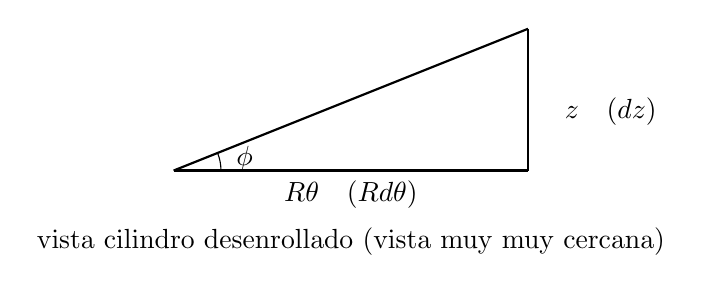
\begin{tikzpicture}[scale=1.5]
    % --- TRIÁNGULO (cilindro desenrollado) ---
    \draw[thick] (0,0) -- (3,1.2); % hipotenusa
    \draw[thick] (0,0) -- (3,0);   % base
    \draw[thick] (3,0) -- (3,1.2); % lado
    % --- ÁNGULO PHI ---
    \draw[dashed] (0,0) -- (0.8,0);
    \draw[dashed] (0,0) -- (0.8,0.32);
    \draw[-] (0.4,0) arc (0:21:0.4);
    \node at (0.6,0.1) {$\phi$};
    % --- ETIQUETAS ---
    \node at (1.5,-0.6) {vista cilindro desenrollado (vista muy muy cercana)};
    \node at (3.7,0.5) {$z\quad(dz)$};
    \node at (1.5,-0.2) {$R\theta \quad(Rd\theta)$};
\end{tikzpicture}
\end{center}
$$\tan(\phi)=\dfrac{z}{R\theta}=\dfrac{dz}{Rd\theta}\longrightarrow z=R\theta\tan(\phi)$$

\patotruco{Como $\phi$ es constante, $z$ queda amarrado a $\theta$ y todo el movimiento depende de una única función $\theta(t)$. Además, en cilíndricas la base se deriva directo: $\dot{\vec{e}}_r=\dot\theta\vec{e}_\theta$ y $\dot{\vec{e}}_\theta=-\dot\theta\vec{e}_r$ (el ``trucazo'', que es el teorema del transporte ya resuelto).}

\textbf{Velocidad}\\
Como se sabe, la velocidad es la derivada temporal de la posición desde un punto fijo.
$$\marc{\vec{v}_P}{N}=\der{\vec{r}_{P}}{N}=\der{(R\vec{e}_r+R)}{N}= R\der{\vec{e}_r}{N}+R\dot\theta\tan(\phi)\vec{e}_z$$
En este caso no es necesario utilizar teorema del transporte porque usamos el trucazo.\\
Derivadas temporales de $\vec{e}_r$ y $\vec{e}_\theta$
$$\transport{\vec{e}_r}{N}{A}=\dot\theta\vec{e}_z\times\vec{e}_r=\dot\theta\vec{e}_\theta $$
$$\transport{\vec{e}_\theta}{N}{A}=\dot\theta\vec{e}_z\times\vec{e}_\theta=-\dot\theta\vec{e}_r $$
y finalmente
$$\marc{\vec{v}_P}{N}=R\dot\theta\vec{e}_\theta+R\dot\theta\tan(\phi)\vec{e}_z$$

\textbf{Aceleración}\\
Al igual que antes podemos simplemente derivar la velocidad para obtener la aceleración.
$$\marc{\vec{a}_P}{N}=\der{\marc{\vec{v}_P}{N}{}}{N}{}=\der{\left(R\dot\theta\vec{e}_\theta+R\dot\theta\tan(\phi)\vec{e}_z\right)}{N}{}=(-R\dot\theta^2)\vec{e}_r+ R\ddot\theta\vec{e}_{\theta}+R\ddot\theta\tan(\phi)\vec{e}_z$$

\textbf{Longitud de arco}\\
La longitud de arco se define como la distancia que recorre la partícula en un lapso de tiempo. Para esto es muy útil saber cuánto recorre en un tiempo ínfimo y se multiplica por el tiempo, así se suma
$$ds=\|\vec{v}_p\|dt\longrightarrow s-s_0=\int\sqrt{R^2\dot\theta^2(1+\tan^2(\phi))}=\int R\dot\theta\sec(\phi)dt$$
Hacemos un cambio de variable, asumiendo que $\theta$ es solo creciente o solo decreciente, es decir, $\dot\theta$ no varía de signo
$$s=\int_{t_0}^t R\dot\theta\sec(\phi)dt\longrightarrow\int_{\theta_0}^\theta R\sec\phi \,\text{d}\theta=R(\theta-\theta_0)\sec(\phi)$$
\respuesta{$\displaystyle s=R\,\theta\sec(\phi)\quad(\theta_0=0)$}
\end{solucion}

\subsubsection{Partícula en mesa circular}
Una partícula, denotada como $P$, se desliza sobre una mesa circular como se muestra en la Figura \ref{fig:masa_circular}. La posición de la partícula se conoce en términos del radio $r$ y el ángulo $\theta$, donde $r$ se mide desde el centro de la mesa en el punto $O$ y $\theta$ se mide en relación con la dirección de $\overline{OQ}$, donde $Q$ es un punto en la circunferencia de la mesa. Sabiendo que la mesa rota con una velocidad angular constante $\Omega$, utilizando el "Teorema de Transporte", determine lo siguiente para un observador en un marco de referencia fijo:

\begin{enumerate}
    \item Los marcos de referencia y sistemas de coordenadas adecuados para describir el movimiento.
    \item El vector posición de la partícula $P$ respecto al centro $O$.
    \item Los vectores de velocidad y aceleración de la partícula $P$ respecto al suelo.
\end{enumerate}

\begin{figure}[!ht]
    \centering
    \begin{tikzpicture}[>=Latex, scale=1.8]
        % --- Parámetros Geométricos ---
        \def\R{1.8}          % Radio de la mesa
        \def\rPos{1.1}        % Distancia radial de P
        \def\angQ{30}         % Orientación de la línea de referencia Q
        \def\thetaAng{40}     % Ángulo theta relativo a OQ

        % --- 1. Mesa Circular ---
        \shadedraw[inner color=white, outer color=gray!40, draw=black, thick] (0,0) circle (\R);
        \filldraw (0,0) circle (1.5pt) node[below left] {$O$};

        % --- 2. Referencia rotatoria en la mesa (OQ) ---
        \coordinate (Q) at (\angQ:\R);
        \draw[thick, dashed] (0,0) -- (Q) node[right] {$Q$};
        
        % --- 3. Posición de la partícula P ---
        % El ángulo absoluto en el dibujo es angQ + thetaAng
        \coordinate (P) at ({\angQ + \thetaAng}:\rPos);
        \draw[->, thick] (0,0) -- (P) node[midway, left] {$r$};
        \filldraw (P) circle (2pt) node[right, xshift=2pt] {$P$};

        % --- 4. Representación del Ángulo Theta ---
        \draw[->] (\angQ:0.7) arc (\angQ:{\angQ+\thetaAng}:0.7);
        \node at ({\angQ + 0.5*\thetaAng}:0.9) {$\theta$};

        % --- 5. Velocidad angular Omega de la mesa ---
        \draw[->, thick] (220:0.4) arc (220:500:0.4);
        \node[below] at (0, -0.45) {$\Omega$};

    \end{tikzpicture}
    \caption{Esquema de una partícula $P$ moviéndose sobre una mesa circular que rota con una velocidad angular constante $\Omega$.}
    \label{fig:masa_circular}
\end{figure}

\ifmostrarSolucion
\begin{tcolorbox}[title=Barra articulada a argolla circular,breakable]
\end{tcolorbox}
\fi

% =========================================================================
% Capítulo 1: Cinemática
% Tema 01: Coordenadas cilíndricas
% Problema 11: Disco en eje giratorio horizontal
% =========================================================================
\subsubsection{Disco en eje giratorio horizontal}

Un disco circular de radio $R$ se une a un eje giratorio de longitud $L$, como se muestra en la Figura \ref{fig:disco_eje_horizontal}. El eje gira respecto de la dirección horizontal con una velocidad angular constante $\Omega$ con respecto al suelo. El disco, a su vez, gira libremente en torno a su centro en el punto $O$. El ángulo $\theta$ describe la posición de un punto $P$ ubicado en el borde del disco relativo al centro del mismo. Utilizando los parámetros indicados, realice lo siguiente:

\begin{enumerate}
    \item Defina los marcos de referencia y los sistemas de coordenadas adecuados para describir el movimiento del sistema desde la perspectiva del suelo.
    \item Determine el vector posición del punto $P$ respecto al punto de apoyo $A$.
    \item Obtenga las expresiones para los vectores de velocidad angular y aceleración angular del eje y del disco.
    \item Calcule los vectores de velocidad y aceleración del punto $P$ respecto al suelo.
\end{enumerate}

\begin{figure}[!ht]
    \centering
    \begin{tikzpicture}[>=Latex, scale=1.8]
        % --- Parámetros Geométricos ---
        \def\L{3.2}          % Longitud del eje
        \def\R{1.1}          % Radio del disco
        \def\thetaAng{45}    % Ángulo theta para el punto P
        \def\BarThickness{0.06} % Grosor de la barra

        % --- Coordenadas ---
        \coordinate (A) at (0,0);
        \coordinate (O) at (\L,0);
        \coordinate (P) at ($ (O) + ({90-\thetaAng}:\R) $);

        % --- 1. Soporte en A ---
        \fill[pattern=north east lines] (-0.3, -0.4) rectangle (0.3, -0.3);
        \draw[thick] (-0.3, -0.3) -- (0.3, -0.3);
        \draw[thin] (A) -- (-0.15, -0.3);
        \draw[thin] (A) -- (0.15, -0.3);
        
        % Articulación A (Gris oscuro)
        \filldraw[fill=gray!80, draw=black] (A) circle (1.8pt) node[below left] {$A$};
    \shadedraw[inner color=white, outer color=gray!40, draw=black, thick] (O) circle (\R);
        % --- 2. Eje Giratorio (Barra L) ---
        \begin{scope}
            \shadedraw[inner color=white, outer color=gray!30, draw=black, rounded corners=2pt] 
                (0, -\BarThickness) rectangle (\L+0.1, \BarThickness);
        \end{scope}
        
        % Velocidad angular Omega
        \draw[->, thick] (1.2, 0.4) arc (60:300:0.2 and 0.4);
        \node[above] at (1.2, 0.4) {$\Omega$};
        
        % Cota de longitud L
        \draw[<->] (0, -0.6) -- (\L, -0.6) node[midway, fill=white] {$L$};
        \draw[dotted] (0, -0.1) -- (0, -0.7);
        \draw[dotted] (\L, -0.1) -- (\L, -0.7);

        % --- 3. Disco en O ---
        
        \draw[dashed] (O) -- ($(O) + (0, \R)$); % Referencia vertical
        
        % Radio R y Ángulo Theta
        \draw[->] (O) -- (P) node[midway, right] {$R$};
        \draw[->] ($(O) + (0, 0.5)$) arc (90:{90-\thetaAng}:0.5);
        \node at ($ (O) + (70:0.75) $) {$\theta$};

        % Articulación O (Gris oscuro)
        \filldraw[fill=gray!80, draw=black] (O) circle (1.2pt) node[above left, xshift=-2pt] {$O$};
        
        % Punto P
        \filldraw (P) circle (1.5pt) node[above right] {$P$};

    \end{tikzpicture}
    \caption{Representación esquemática de un disco de radio $R$ montado en un eje giratorio horizontal de longitud $L$.}
    \label{fig:disco_eje_horizontal}
\end{figure}

% --- SOLUCIÓN ---------------------------------------------------------------
\begin{solucion}{Disco en eje giratorio horizontal}
Lo primero que hacemos es definir los marcos de referencia, con los cuales trabajaremos durante el ejercicio.
\begin{itemize}
    \item $\mathcal{N}$ Suelo (Inercial) $\{\vec{E_x},\vec{E_y},\vec{E_z}\}$
    \item $\mathcal{A}$ Barra $AO$ $\{\vec{e_x},\vec{e_y},\vec{e_z}\}$
    \item $\mathcal{B}$ Disco  $\{\vec{e}_r,\vec{e}_\theta,\vec{e}_z\}$
\end{itemize}

\begin{center}
        \begin{tikzpicture}[>=Latex, scale=1.8]
        % --- Parámetros Geométricos ---
        \def\L{3.2}          % Longitud del eje
        \def\R{1.1}          % Radio del disco
        \def\thetaAng{45}    % Ángulo theta para el punto P
        \def\BarThickness{0.06} % Grosor de la barra

        % --- Coordenadas ---
        \coordinate (A) at (0,0);
        \coordinate (O) at (\L,0);
        \coordinate (P) at ($ (O) + ({90-\thetaAng}:\R) $);

        % --- 1. Soporte en A ---
        \fill[pattern=north east lines] (-0.3, -0.4) rectangle (0.3, -0.3);
        \draw[thick] (-0.3, -0.3) -- (0.3, -0.3);
        \draw[thin] (A) -- (-0.15, -0.3);
        \draw[thin] (A) -- (0.15, -0.3);
        
        % Articulación A (Gris oscuro)
        \filldraw[fill=gray!80, draw=black] (A) circle (1.8pt) node[below left] {$A$};
    \shadedraw[inner color=white, outer color=gray!40, draw=black, thick] (O) circle (\R);
        % --- 2. Eje Giratorio (Barra L) ---
        \begin{scope}
            \shadedraw[inner color=white, outer color=gray!30, draw=black, rounded corners=2pt] 
                (0, -\BarThickness) rectangle (\L+0.1, \BarThickness);
        \end{scope}
        
        % Velocidad angular Omega
        \draw[->, thick] (1.2, 0.4) arc (60:300:0.2 and 0.4);
        \node[above] at (1.2, 0.4) {$\Omega$};
        
        % Cota de longitud L
        \draw[<->] (0, -0.6) -- (\L, -0.6) node[midway, below] {$L$};
        \draw[dotted] (0, -0.1) -- (0, -0.7);
        \draw[dotted] (\L, -0.1) -- (\L, -0.7);

        % --- 3. Disco en O ---
        
        \draw[dashed] (O) -- ($(O) + (0, \R)$); % Referencia vertical
        
        % Radio R y Ángulo Theta
        \draw[->] (O) -- (P) node[midway, right] {$R$};
        \draw[->] ($(O) + (0, 0.5)$) arc (90:{90-\thetaAng}:0.5);
        \node at ($ (O) + (70:0.75) $) {$\theta$};

        % Articulación O (Gris oscuro)
        \filldraw[fill=gray!80, draw=black] (O) circle (1.2pt) node[above left, xshift=-2pt] {$O$};
        
        % Punto P
        \filldraw (P) circle (1.5pt) node[above right] {$P$};

        %aqui van los vectores
        \draw[->, thick, red] (0,0)--++(0.5,0) node[below] {$\vec{E}_y$};
        \draw[->, thick, red] (0,0)--++(0,0.5) node[above] {$\vec{E}_z$};
        
        %aqui van los vectores
        \draw[->, thick, blue] (\L,0)--++(0.7,0) node[below] {$\vec{e}_x$};
        \draw[->, thick, blue] (\L,0)--++(0,0.7) node[above] {$\vec{e}_y$};
        %aqui van los vectores
        \draw[->, thick, green] (\L,0)--++(45:0.7) node[above] {$\vec{e}_r$};
        \draw[->, thick, green] (\L,0)--++(-45:0.7) node[below] {$\vec{e}_\theta$};

    \end{tikzpicture}
\end{center}
\end{solucion}


% =========================================================================
% Capítulo 1: Cinemática
% Tema 01: Coordenadas cilíndricas
% Problema 13: Disco rotante
% =========================================================================
% NOTA: el archivo original estaba vacío; el enunciado se reconstruyó a
% partir de los datos de la solución. Revisar.
\subsubsection{Disco rotante}
Un disco gira con velocidad angular constante $\Omega$ alrededor de su eje, que es fijo al
suelo. Un punto $P$ se mueve radialmente sobre el disco, alejándose del centro con rapidez
constante $v$ relativa al disco, de modo que $r(t) = r_0 + vt$ y $\theta(t) = \Omega t$.
Determine, para un observador fijo al suelo:
\begin{enumerate}
    \item La velocidad del punto $P$.
    \item La aceleración del punto $P$.
    \item Las componentes de la aceleración y su interpretación física.
\end{enumerate}

% --- SOLUCIÓN ---------------------------------------------------------------
\begin{solucion}{Disco rotante}
\subsubsection*{Pregunta 1: Velocidad del punto P}

En coordenadas cilíndricas, la posición del punto es:
$$\vec{r} = r(t) \, \hat{e}_r + z \, \hat{e}_z$$

Con $r(t) = r_0 + vt$ (movimiento radial constante) y $\theta(t) = \Omega t$ (rotación a velocidad angular constante).

La velocidad en coordenadas cilíndricas es:
$$\vec{v} = \dot{r} \, \hat{e}_r + r \dot{\theta} \, \hat{e}_\theta + \dot{z} \, \hat{e}_z$$

Sustituyendo nuestras funciones:
\begin{equation}
\boxed{\vec{v} = v \, \hat{e}_r + (r_0 + vt) \Omega \, \hat{e}_\theta}
\end{equation}

Interpretación:
\begin{itemize}
    \item \textbf{Componente radial}: $v_r = v$ (constante, movimiento hacia afuera)
    \item \textbf{Componente transversal}: $v_\theta = (r_0 + vt) \Omega$ (aumenta con el tiempo)
    \item \textbf{Magnitud de velocidad}: $|\vec{v}| = \sqrt{v^2 + [(r_0 + vt) \Omega]^2}$
\end{itemize}

\subsubsection*{Pregunta 2: Aceleración del punto P}

La aceleración en coordenadas cilíndricas es:
$$\vec{a} = (\ddot{r} - r\dot{\theta}^2) \hat{e}_r + (r\ddot{\theta} + 2\dot{r}\dot{\theta}) \hat{e}_\theta + \ddot{z} \, \hat{e}_z$$

Con nuestras funciones:
\begin{itemize}
    \item $\dot{r} = v$ (velocidad radial constante)
    \item $\ddot{r} = 0$ (aceleración radial nula)
    \item $\dot{\theta} = \Omega$ (velocidad angular constante)
    \item $\ddot{\theta} = 0$ (aceleración angular nula)
    \item $r = r_0 + vt$
\end{itemize}

Sustituyendo:
\begin{equation}
\vec{a} = [0 - (r_0 + vt)\Omega^2] \hat{e}_r + [0 + 2v\Omega] \hat{e}_\theta
\end{equation}

\begin{equation}
\boxed{\vec{a} = -(r_0 + vt) \Omega^2 \, \hat{e}_r + 2v\Omega \, \hat{e}_\theta}
\end{equation}

\subsubsection*{Pregunta 3: Componentes de Aceleración}

\paragraph{Componente Radial (Centrípeta)}
$$a_r = -(r_0 + vt) \Omega^2$$

Esta es la aceleración \textbf{centrípeta}: negativa (apunta hacia el centro), proporcional a la distancia radial, y proporcional al cuadrado de la velocidad angular. Su magnitud aumenta linealmente con el tiempo.

\paragraph{Componente Transversal (Coriolis)}
$$a_\theta = 2v\Omega$$

Esta es la aceleración de \textbf{Coriolis}: es constante, proporcional a la velocidad radial $v$ y a la velocidad angular $\Omega$. Representa el cambio de dirección de la velocidad debido a la rotación del sistema.

\paragraph{Componente Axial}
$$a_z = 0$$

No hay movimiento en la dirección axial (perpendicular al disco).

\paragraph{Magnitud Total}
\begin{equation}
|\vec{a}| = \sqrt{[(r_0 + vt) \Omega^2]^2 + (2v\Omega)^2}
\end{equation}

\paragraph{Interpretación Física}

El término centrípeto $-(r_0 + vt) \Omega^2$ es necesario para mantener el punto en una trayectoria circular alrededor del eje mientras se aleja del centro. El término de Coriolis $2v\Omega$ resulta del hecho de que la velocidad del punto en la dirección transversal $v_\theta = (r_0 + vt) \Omega$ cambia continuamente debido al movimiento radial: conforme el punto se aleja del eje, su velocidad tangencial aumenta, requiriendo una aceleración tangencial.
\end{solucion}

% =========================================================================
% Capítulo 1: Cinemática
% Tema 01: Coordenadas cilíndricas
% Problema 14: Movimiento en Espiral Logarítmica
% =========================================================================
\subsubsection{Movimiento en Espiral Logarítmica}

Un punto $P$ sigue una trayectoria en espiral logarítmica descrita en coordenadas cilíndricas por:
$$r(\theta) = r_0 e^{-k\theta}$$

donde $r_0$ es el radio inicial, $k$ es una constante positiva de amortiguamiento, y $\theta$ es el ángulo azimutal. El punto se desplaza de modo que su velocidad angular es constante: $\dot{\theta} = \omega_0$.

\begin{enumerate}
    \item Expresar la velocidad del punto en coordenadas cilíndricas.
    \item Calcular la aceleración del punto.
    \item Demostrar que la rapidez (magnitud de velocidad) decrece exponencialmente con el tiempo.
\end{enumerate}

\begin{figure}[!ht]
    \centering
    \begin{tikzpicture}[>=Latex, scale=1.6]

        % --- CONFIGURACIÓN DE PARÁMETROS ---
        \def\ro{2.5}      % Radio inicial r0 [cm]
        \def\k{0.15}      % Constante de amortiguamiento k
        \def\w{1}         % Escala de la espiral

        % --- SOPORTES Y ELEMENTOS FIJOS ---
        % Origen
        \coordinate (O) at (0,0);
        \filldraw (O) circle (1.5pt) node[above left] {$O$};

        % --- GEOMETRÍA PRINCIPAL ---
        % Espiral logarítmica (dibujada como varios puntos conectados)
        \draw[thick, azul]
            plot[parametric, samples=100, domain=0:3*pi]
            ({0.8*\ro*exp(-\k*\x/pi)*cos(\x r)}, {0.8*\ro*exp(-\k*\x/pi)*sin(\x r)});

        % --- SISTEMAS DE COORDENADAS ---
        % Ejes de referencia
        \draw[->, thick] (O) -- (3, 0) node[right, font=\small] {$x$};
        \draw[->, thick] (O) -- (0, 3) node[above, font=\small] {$y$};

        % --- PUNTOS Y COORDENADAS ---
        % Punto inicial en la espiral (t=0)
        \coordinate (P0) at (0.8*\ro, 0);
        \filldraw[fill=white, thick] (P0) circle (2.5pt);
        \filldraw (P0) circle (1pt) node[right, font=\small] {$P(t=0)$};

        % Punto en tiempo intermedio
        \coordinate (Pm) at ({0.8*\ro*exp(-\k*pi/2)*cos(pi/2 r)}, {0.8*\ro*exp(-\k*pi/2)*sin(pi/2 r)});
        \filldraw[fill=white, thick] (Pm) circle (2pt);
        \filldraw (Pm) circle (1pt);

        % Punto cerca del origen (t grande)
        \coordinate (Pf) at ({0.8*\ro*exp(-\k*3*pi)*cos(3*pi r)}, {0.8*\ro*exp(-\k*3*pi)*sin(3*pi r)});
        \filldraw[fill=white, thick] (Pf) circle (2pt);
        \filldraw (Pf) circle (1pt) node[left, font=\small] {$P(t \to \infty)$};

        % --- VECTORES Y FUERZAS ---
        % Vector de velocidad en el punto inicial
        % Velocidad radial (hacia adentro) + velocidad tangencial
        \draw[->, thick, myred] (P0) -- ($(P0) + (-0.4, 0)$) node[below, font=\small, color=myred] {$\vec{v}_r$};
        \draw[->, thick, orange] (P0) -- ($(P0) + (0, 0.5)$) node[above, font=\small, color=orange] {$\vec{v}_\theta$};

        % Vector velocidad total (resultante)
        \draw[->, thick, gris1] (P0) -- ($(P0) + (-0.4, 0.5)$) node[above right, font=\small, color=gris1] {$\vec{v}$};

        % --- ANOTACIONES Y ETIQUETAS ---
        % Ángulo theta en un punto
        \draw[dashed, gray] (0, 0) -- (Pm);
        \draw[->, dashed, gray] (0.5, 0) arc (0:90:0.5);
        \node at (0.6, 0.4) [font=\small] {$\theta$};

        % Radio en el punto inicial
        \draw[<->, thin, gray] (0, -0.35) -- (P0) node[midway, below, font=\small] {$r_0$};

        % Etiqueta
        \node[font=\footnotesize] at (1.5, -2) {Espiral logarítmica: $r(\theta) = r_0 e^{-k\theta}$};

    \end{tikzpicture}
    \caption{Trayectoria en espiral logarítmica con velocidad descompuesta en componentes radial y transversal}
    \label{fig:c1_e01_p05_espiral}
\end{figure}

% --- SOLUCIÓN ---------------------------------------------------------------
\begin{solucion}{Espiral logarítmica}
\subsubsection*{Pregunta 1: Velocidad en Coordenadas Cilíndricas}

Dado que $\theta(t) = \omega_0 t$ (velocidad angular constante), tenemos $\dot{\theta} = \omega_0$ y $\ddot{\theta} = 0$.

De la ecuación de la espiral $r(\theta) = r_0 e^{-k\theta}$, obtenemos $r(t) = r_0 e^{-k\omega_0 t}$.

Derivando respecto al tiempo:
$$\dot{r} = r_0 \cdot (-k\omega_0) e^{-k\omega_0 t} = -k\omega_0 \cdot r_0 e^{-k\omega_0 t} = -k\omega_0 \cdot r(t)$$

La velocidad en coordenadas cilíndricas es:
$$\vec{v} = \dot{r} \, \hat{e}_r + r\dot{\theta} \, \hat{e}_\theta$$

Sustituyendo:
\begin{equation}
\boxed{\vec{v} = -k\omega_0 r(t) \, \hat{e}_r + r(t) \omega_0 \, \hat{e}_\theta = \omega_0 r(t) \left[ -k \, \hat{e}_r + \hat{e}_\theta \right]}
\end{equation}

\subsubsection*{Pregunta 2: Aceleración del Punto}

La aceleración en coordenadas cilíndricas es:
$$\vec{a} = (\ddot{r} - r\dot{\theta}^2) \hat{e}_r + (r\ddot{\theta} + 2\dot{r}\dot{\theta}) \hat{e}_\theta$$

Calculamos las derivadas necesarias:
\begin{itemize}
    \item $\dot{r} = -k\omega_0 r(t)$
    \item $\ddot{r} = -k\omega_0 \dot{r} = -k\omega_0 \cdot (-k\omega_0 r) = k^2 \omega_0^2 r(t)$
    \item $\dot{\theta} = \omega_0$
    \item $\ddot{\theta} = 0$
\end{itemize}

Componente radial:
$$a_r = \ddot{r} - r\dot{\theta}^2 = k^2 \omega_0^2 r - r \omega_0^2 = (k^2 - 1) \omega_0^2 r$$

Componente transversal:
$$a_\theta = r \cdot 0 + 2 \cdot (-k\omega_0 r) \cdot \omega_0 = -2k\omega_0^2 r$$

La aceleración total es:
\begin{equation}
\boxed{\vec{a} = (k^2 - 1) \omega_0^2 r(t) \, \hat{e}_r - 2k\omega_0^2 r(t) \, \hat{e}_\theta}
\end{equation}

o, factorizando:
\begin{equation}
\vec{a} = \omega_0^2 r(t) \left[ (k^2 - 1) \hat{e}_r - 2k \, \hat{e}_\theta \right]
\end{equation}

\paragraph{Análisis de la Aceleración}

\begin{itemize}
    \item Si $k < 1$: La componente radial apunta hacia afuera (positiva), aunque el punto se acerca al origen. Esto ocurre porque la velocidad radial disminuye en magnitud; el cambio de velocidad radial implica aceleración hacia afuera.
    \item Si $k = 1$: La componente radial es cero; solo existe aceleración transversal (similar a movimiento circular uniforme de radio variable).
    \item Si $k > 1$: La componente radial apunta hacia adentro, acelerando la convergencia.
    \item La componente transversal $a_\theta = -2k\omega_0^2 r$ siempre apunta en dirección negativa (contraria a la velocidad angular), ralentizando la rotación.
\end{itemize}

\subsubsection*{Pregunta 3: Rapidez Exponencial Decreciente}

La rapidez (magnitud de velocidad) es:
$$v = |\vec{v}| = \sqrt{(\dot{r})^2 + (r\dot{\theta})^2} = \sqrt{k^2\omega_0^2 r^2 + r^2 \omega_0^2}$$

$$v = \omega_0 r \sqrt{k^2 + 1} = \omega_0 \sqrt{k^2 + 1} \cdot r_0 e^{-k\omega_0 t}$$

\begin{equation}
\boxed{v(t) = v_0 e^{-k\omega_0 t}}
\end{equation}

donde $v_0 = \omega_0 r_0 \sqrt{k^2 + 1}$ es la rapidez inicial.

\paragraph{Demostración}

La rapidez disminuye exponencialmente con constante de tiempo $\tau = 1/(k\omega_0)$. Conforme $t \to \infty$:
- $r(t) \to 0$ (el punto converge al origen)
- $v(t) \to 0$ (la velocidad tiende a cero)
- El punto completa infinitas revoluciones alrededor del origen en tiempo finito, pero su velocidad disminuye exponencialmente.

Este comportamiento es típico de sistemas disipativos donde la energía cinética se reduce continuamente.
\end{solucion}


\newpage
\subsection{Soluciones del Tema 01}

% =========================================================================
% Solución: C1_E01_P04 - Disco Rotante con Punto en Movimiento Radial
% =========================================================================

\begin{sol}[Tema: Cinemática en Coordenadas Cilíndricas - Disco Rotante]

\subsubsection*{Pregunta 1: Velocidad del punto P}

En coordenadas cilíndricas, la posición del punto es:
$$\vec{r} = r(t) \, \hat{e}_r + z \, \hat{e}_z$$

Con $r(t) = r_0 + vt$ (movimiento radial constante) y $\theta(t) = \Omega t$ (rotación a velocidad angular constante).

La velocidad en coordenadas cilíndricas es:
$$\vec{v} = \dot{r} \, \hat{e}_r + r \dot{\theta} \, \hat{e}_\theta + \dot{z} \, \hat{e}_z$$

Sustituyendo nuestras funciones:
\begin{equation}
\boxed{\vec{v} = v \, \hat{e}_r + (r_0 + vt) \Omega \, \hat{e}_\theta}
\end{equation}

Interpretación:
\begin{itemize}
    \item \textbf{Componente radial}: $v_r = v$ (constante, movimiento hacia afuera)
    \item \textbf{Componente transversal}: $v_\theta = (r_0 + vt) \Omega$ (aumenta con el tiempo)
    \item \textbf{Magnitud de velocidad}: $|\vec{v}| = \sqrt{v^2 + [(r_0 + vt) \Omega]^2}$
\end{itemize}

\subsubsection*{Pregunta 2: Aceleración del punto P}

La aceleración en coordenadas cilíndricas es:
$$\vec{a} = (\ddot{r} - r\dot{\theta}^2) \hat{e}_r + (r\ddot{\theta} + 2\dot{r}\dot{\theta}) \hat{e}_\theta + \ddot{z} \, \hat{e}_z$$

Con nuestras funciones:
\begin{itemize}
    \item $\dot{r} = v$ (velocidad radial constante)
    \item $\ddot{r} = 0$ (aceleración radial nula)
    \item $\dot{\theta} = \Omega$ (velocidad angular constante)
    \item $\ddot{\theta} = 0$ (aceleración angular nula)
    \item $r = r_0 + vt$
\end{itemize}

Sustituyendo:
\begin{equation}
\vec{a} = [0 - (r_0 + vt)\Omega^2] \hat{e}_r + [0 + 2v\Omega] \hat{e}_\theta
\end{equation}

\begin{equation}
\boxed{\vec{a} = -(r_0 + vt) \Omega^2 \, \hat{e}_r + 2v\Omega \, \hat{e}_\theta}
\end{equation}

\subsubsection*{Pregunta 3: Componentes de Aceleración}

\paragraph{Componente Radial (Centrípeta)}
$$a_r = -(r_0 + vt) \Omega^2$$

Esta es la aceleración \textbf{centrípeta}: negativa (apunta hacia el centro), proporcional a la distancia radial, y proporcional al cuadrado de la velocidad angular. Su magnitud aumenta linealmente con el tiempo.

\paragraph{Componente Transversal (Coriolis)}
$$a_\theta = 2v\Omega$$

Esta es la aceleración de \textbf{Coriolis}: es constante, proporcional a la velocidad radial $v$ y a la velocidad angular $\Omega$. Representa el cambio de dirección de la velocidad debido a la rotación del sistema.

\paragraph{Componente Axial}
$$a_z = 0$$

No hay movimiento en la dirección axial (perpendicular al disco).

\paragraph{Magnitud Total}
\begin{equation}
|\vec{a}| = \sqrt{[(r_0 + vt) \Omega^2]^2 + (2v\Omega)^2}
\end{equation}

\paragraph{Interpretación Física}

El término centrípeto $-(r_0 + vt) \Omega^2$ es necesario para mantener el punto en una trayectoria circular alrededor del eje mientras se aleja del centro. El término de Coriolis $2v\Omega$ resulta del hecho de que la velocidad del punto en la dirección transversal $v_\theta = (r_0 + vt) \Omega$ cambia continuamente debido al movimiento radial: conforme el punto se aleja del eje, su velocidad tangencial aumenta, requiriendo una aceleración tangencial.

\end{sol}


\newpage
% =========================================================================
% Solución: C1_E01_P05 - Movimiento en Espiral Logarítmica
% =========================================================================

\begin{sol}[Tema: Cinemática en Coordenadas Cilíndricas - Espiral Logarítmica]

\subsubsection*{Pregunta 1: Velocidad en Coordenadas Cilíndricas}

Dado que $\theta(t) = \omega_0 t$ (velocidad angular constante), tenemos $\dot{\theta} = \omega_0$ y $\ddot{\theta} = 0$.

De la ecuación de la espiral $r(\theta) = r_0 e^{-k\theta}$, obtenemos $r(t) = r_0 e^{-k\omega_0 t}$.

Derivando respecto al tiempo:
$$\dot{r} = r_0 \cdot (-k\omega_0) e^{-k\omega_0 t} = -k\omega_0 \cdot r_0 e^{-k\omega_0 t} = -k\omega_0 \cdot r(t)$$

La velocidad en coordenadas cilíndricas es:
$$\vec{v} = \dot{r} \, \hat{e}_r + r\dot{\theta} \, \hat{e}_\theta$$

Sustituyendo:
\begin{equation}
\boxed{\vec{v} = -k\omega_0 r(t) \, \hat{e}_r + r(t) \omega_0 \, \hat{e}_\theta = \omega_0 r(t) \left[ -k \, \hat{e}_r + \hat{e}_\theta \right]}
\end{equation}

\subsubsection*{Pregunta 2: Aceleración del Punto}

La aceleración en coordenadas cilíndricas es:
$$\vec{a} = (\ddot{r} - r\dot{\theta}^2) \hat{e}_r + (r\ddot{\theta} + 2\dot{r}\dot{\theta}) \hat{e}_\theta$$

Calculamos las derivadas necesarias:
\begin{itemize}
    \item $\dot{r} = -k\omega_0 r(t)$
    \item $\ddot{r} = -k\omega_0 \dot{r} = -k\omega_0 \cdot (-k\omega_0 r) = k^2 \omega_0^2 r(t)$
    \item $\dot{\theta} = \omega_0$
    \item $\ddot{\theta} = 0$
\end{itemize}

Componente radial:
$$a_r = \ddot{r} - r\dot{\theta}^2 = k^2 \omega_0^2 r - r \omega_0^2 = (k^2 - 1) \omega_0^2 r$$

Componente transversal:
$$a_\theta = r \cdot 0 + 2 \cdot (-k\omega_0 r) \cdot \omega_0 = -2k\omega_0^2 r$$

La aceleración total es:
\begin{equation}
\boxed{\vec{a} = (k^2 - 1) \omega_0^2 r(t) \, \hat{e}_r - 2k\omega_0^2 r(t) \, \hat{e}_\theta}
\end{equation}

o, factorizando:
\begin{equation}
\vec{a} = \omega_0^2 r(t) \left[ (k^2 - 1) \hat{e}_r - 2k \, \hat{e}_\theta \right]
\end{equation}

\paragraph{Análisis de la Aceleración}

\begin{itemize}
    \item Si $k < 1$: La componente radial apunta hacia afuera (positiva), aunque el punto se acerca al origen. Esto ocurre porque la velocidad radial disminuye en magnitud; el cambio de velocidad radial implica aceleración hacia afuera.
    \item Si $k = 1$: La componente radial es cero; solo existe aceleración transversal (similar a movimiento circular uniforme de radio variable).
    \item Si $k > 1$: La componente radial apunta hacia adentro, acelerando la convergencia.
    \item La componente transversal $a_\theta = -2k\omega_0^2 r$ siempre apunta en dirección negativa (contraria a la velocidad angular), ralentizando la rotación.
\end{itemize}

\subsubsection*{Pregunta 3: Rapidez Exponencial Decreciente}

La rapidez (magnitud de velocidad) es:
$$v = |\vec{v}| = \sqrt{(\dot{r})^2 + (r\dot{\theta})^2} = \sqrt{k^2\omega_0^2 r^2 + r^2 \omega_0^2}$$

$$v = \omega_0 r \sqrt{k^2 + 1} = \omega_0 \sqrt{k^2 + 1} \cdot r_0 e^{-k\omega_0 t}$$

\begin{equation}
\boxed{v(t) = v_0 e^{-k\omega_0 t}}
\end{equation}

donde $v_0 = \omega_0 r_0 \sqrt{k^2 + 1}$ es la rapidez inicial.

\paragraph{Demostración}

La rapidez disminuye exponencialmente con constante de tiempo $\tau = 1/(k\omega_0)$. Conforme $t \to \infty$:
- $r(t) \to 0$ (el punto converge al origen)
- $v(t) \to 0$ (la velocidad tiende a cero)
- El punto completa infinitas revoluciones alrededor del origen en tiempo finito, pero su velocidad disminuye exponencialmente.

Este comportamiento es típico de sistemas disipativos donde la energía cinética se reduce continuamente.

\end{sol}

